\section{Results}
\label{sec:results}
\paragraph{Clean accuracy.} The undefended model reaches 98.8\% test accuracy (600 pairs, AUC $\approx$1.00) and all defenses stay within 98.7--99.2\% (Tab.~\ref{tab:baseline}), so on clean data the filters cost almost nothing.

\paragraph{Non-adaptive attacks versus filters.} Undefended, PGD succeeds on 100\% and FGSM on 79\% of pairs at $\epsilon{=}4$. The filters help partially: the best, $5{\times}5$ median, reduces PGD to 79\% and FGSM to 61\%, and JPEG-30 to 85\%. At $\epsilon{=}8$ no filter helps (PGD ASR 97.6--100\%). These attacks ignore the defense, so these are optimistic numbers for the filters.

\begin{table}[t]
\centering\small
\begin{tabular}{lccccc}
\toprule
Defense & Clean acc. & FGSM$_4$ & PGD$_2$ & PGD$_4$ & PGD$_8$ \\
\midrule
None & 0.988 & 0.788 & 0.855 & 1.000 & 1.000 \\
JPEG-75 & 0.987 & 0.730 & 0.659 & 0.983 & 1.000 \\
JPEG-50 & 0.992 & 0.695 & 0.510 & 0.960 & 0.997 \\
JPEG-30 & 0.987 & 0.633 & 0.333 & 0.852 & 0.993 \\
Gaussian & 0.990 & 0.677 & 0.481 & 0.966 & 1.000 \\
Median 3$\times$3 & 0.988 & 0.737 & 0.687 & 0.983 & 1.000 \\
Median 5$\times$5 & 0.988 & 0.613 & 0.293 & 0.791 & 0.976 \\
4-bit depth & 0.988 & 0.760 & 0.696 & 0.986 & 1.000 \\
\bottomrule
\end{tabular}

\caption{Clean test accuracy and attack success rate (ASR, lower is better) of single-filter defenses against non-adaptive attacks (300 pairs). Subscript = $\epsilon$ in /255.}
\label{tab:baseline}
\end{table}

\paragraph{Detector and fusion.} Tab.~\ref{tab:main} gives ASR for the fused system next to the best single filters. Trained only on FGSM and PGD, the selected boosted-trees detector reduces ASR to $\le$0.02 for FGSM, PGD, CW, DeepFool (whose ASR is only 4\% anyway), other budgets up to $\epsilon{=}4$, and PGD at $\epsilon{=}8$, and to 0.29 for FGSM at $\epsilon{=}8$. It fails on Square: detector AUC is 0.58 and only 8\% of Square pairs are flagged; since Square rarely succeeds at 100 queries (3\% ASR) this is weak evidence, but it does show the detector does not detect every perturbation type. Detector choice matters (Tab.~\ref{tab:det}): LDA is clearly worse than the nonlinear models, which are similar on seen attacks.

\begin{table*}[t]
\centering\small
\begin{tabular}{lcccccc}
\toprule
Attack ($\epsilon{=}4$ unless stated) & None & JPEG-30 & Median-5 & Fused & Flag rate & Det.\ AUC \\
\midrule
FGSM & 0.788 & 0.636 & 0.613 & \textbf{0.020} & 0.97 & 0.994 \\
PGD & 1.000 & 0.859 & 0.791 & \textbf{0.000} & 1.00 & 1.000 \\
\midrule
DeepFool & 0.040 & 0.017 & 0.007 & \textbf{0.000} & 0.96 & 0.991 \\
CW-L2 & 0.663 & 0.168 & 0.121 & \textbf{0.003} & 0.99 & 0.998 \\
Square (black-box) & 0.030 & 0.030 & 0.027 & \textbf{0.024} & 0.08 & 0.580 \\
\midrule
FGSM, $\epsilon{=}2$ & 0.532 & 0.239 & 0.205 & \textbf{0.000} & 1.00 & 0.999 \\
FGSM, $\epsilon{=}8$ & 0.882 & 0.811 & 0.822 & \textbf{0.293} & 0.68 & 0.928 \\
PGD, $\epsilon{=}2$ & 0.855 & 0.333 & 0.293 & \textbf{0.000} & 1.00 & 1.000 \\
PGD, $\epsilon{=}8$ & 1.000 & 0.993 & 0.976 & \textbf{0.013} & 0.99 & 0.999 \\
\midrule
BPDA via JPEG-30 & 0.973 & 0.899 & 0.779 & \textbf{0.000} & 1.00 & 1.000 \\
BPDA via Median-5 & 0.973 & 0.839 & 0.966 & \textbf{0.000} & 1.00 & 0.995 \\
BPDA via Gaussian & 0.987 & 0.899 & 0.926 & \textbf{0.000} & 1.00 & 0.997 \\
Adaptive (all transforms) & 1.000 & 0.933 & 0.926 & \textbf{0.000} & 1.00 & 1.000 \\
Detector-aware adaptive & 1.000 & 0.940 & 0.933 & \textbf{0.000} & 1.00 & 1.000 \\
\bottomrule
\end{tabular}

\caption{ASR of single filters and of the fused system (flagged pairs count as stopped), flag rate on attacked pairs, and detector AUC (boosted trees; clean vs.\ attacked test pairs). Groups: seen / unseen attack / other budget / adaptive (150 pairs). Bold = lowest ASR in the row.}
\label{tab:main}
\end{table*}

\begin{table}[t]
\centering\small
\begin{tabular}{lccccc}
\toprule
Detector & Val AUC & Seen & Unseen & Other $\epsilon$ & Adaptive \\
\midrule
LDA & 0.861 & 0.877 & 0.684 & 0.844 & 0.915 \\
Gaussian Bayes (QDA) & 0.989 & 0.991 & 0.878 & 0.977 & 0.999 \\
RBF-SVM & 0.994 & 0.996 & 0.877 & 0.982 & 1.000 \\
Boosted trees & 0.997 & 0.997 & 0.856 & 0.982 & 0.998 \\
\bottomrule
\end{tabular}

\caption{Mean detector AUC by detector type on attack groups (seen: FGSM, PGD; unseen: DeepFool, CW, Square; other $\epsilon$; adaptive). Val AUC is on seen attacks.}
\label{tab:det}
\end{table}

\paragraph{Adaptive attacks.} Single filters collapse once the attacker knows them: BPDA through JPEG-30 reaches 90\% ASR against JPEG-30 and BPDA through median-5 reaches 97\% against median-5, and the ensemble attack over all transforms reaches 93\% against both JPEG-30 and median-5 (100\% undefended). The fused system flags all of these attacked pairs (AUC 0.995--1.000), including the detector-aware variant that explicitly keeps the embedding stable under the transforms. We stress that this is evidence about two specific attacks and 150 pairs, not a proof: an attacker that optimizes the detector's decision directly was not evaluated.

\begin{figure}[t]
  \centering
  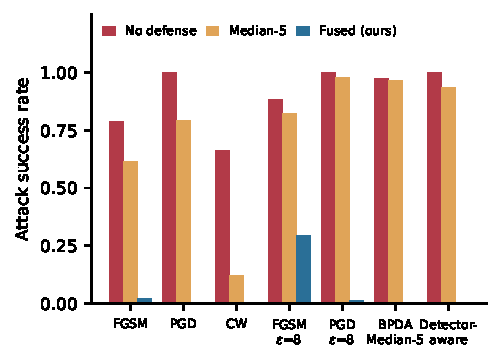
\includegraphics[width=0.98\linewidth]{figures/asr.pdf}
  \caption{ASR for no defense, median-5 and the fused system on selected attacks. Fused bars at 0 are invisible. Adaptive attacks defeat the median filter; the fused system is not beaten by them in our tests.}
  \label{fig:asr}
\end{figure}

\paragraph{Cost of flagging and benign controls.} At the 5\% operating point the system flags \cleanflag\% of clean test pairs and makes \cleanerr\% unflagged errors. A detector could be mistaken for a generic noise detector, so we also feed it benign perturbed inputs: random $\pm4/255$ noise is flagged \noiseflag\% of the time (near the 5\% budget) and plain JPEG-75 images \jpegflag\%, versus 96--100\% for FGSM, PGD, DeepFool, CW and the adaptive attacks (Fig.~\ref{fig:flags}).

\begin{figure}[t]
  \centering
  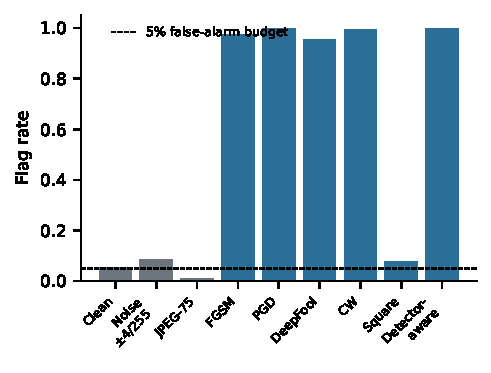
\includegraphics[width=0.98\linewidth]{figures/flags.pdf}
  \caption{Flag rate of the fused system on clean pairs, benign perturbations (grey) and attacks (blue). The dashed line is the 5\% false-alarm budget fixed on validation data.}
  \label{fig:flags}
\end{figure}

\paragraph{Ablation and cost.} Using LDA with $s_0$ plus one transform, the mean AUC over the five non-adaptive attacks is similar for JPEG-75, median and Gaussian (0.78--0.79), slightly lower for JPEG-30 (0.75) and much lower for 4-bit depth (0.53); using all transforms with LDA gives 0.76 (Tab.~\ref{tab:abl}). A forward-selection run (SFFS-style) picked $s_0$, $s_{\text{JPEG-75}}-s_0$, JPEG-75 drift and median drift. The LDA ablation is only indicative because LDA is the weakest detector. Computing the features requires $|\mathcal T|{+}1{=}6$ embeddings per image: \msdet\,ms per pair versus \msbase\,ms for plain verification on our CPU ($\approx$\mscratio$\times$; timings vary between runs), so the defense is training-free and cheap compared with adversarial training, but not free.

\begin{table}[t]
\centering\small
\begin{tabular}{lc}
\toprule
LDA features & Mean AUC (5 non-adaptive attacks) \\
\midrule
$s_0$ + jpeg75 & 0.780 \\
$s_0$ + jpeg30 & 0.745 \\
$s_0$ + median3 & 0.777 \\
$s_0$ + gaussian & 0.788 \\
$s_0$ + bitdepth4 & 0.532 \\
all transforms (LDA) & 0.761 \\
\bottomrule
\end{tabular}

\caption{Ablation: LDA detector with $s_0$ plus one transform's features.}
\label{tab:abl}
\end{table}
